\documentclass[]{article}

\usepackage[utf8]{inputenc} %este pacote serve para digitar em portugues
\usepackage{graphicx}
\usepackage{epigraph}
%opening
\title{Visualização de Informação em Sistemas Científicos}
\author{Luis Gustavo Neves 
\and Prof. Dr. Asla Sá}

\begin{document}

\maketitle

\begin{abstract}

Este trabalho é um estudo sobre a aplicação de técnicas de visualização de informação em sistemas de software voltados para matemática, ciências e engenharias. 

\end{abstract}

\epigraph{"This life's dim windows of the soul
Distorts the heavens from pole to pole
And leads you to believe a lie
When you see with, not through, the eye."}{The Everlasting Gospel, William Blake}

\tableofcontents

\section{Agradecimentos}

\section{Introdução} 

\subsection{Forewords}

Podemos definir a visualização de informação como a comunicação de representações gráficas para criação de um modelo ou imagem mental. O potencial oferecido pela visualização de informação passou por um enorme crescimento nos últimos vinte anos, em função do aperfeiçoamento dos computadores pessoais. Ainda assim, sua essência pode ser observada em exemplos muito anteriores à invenção da computação e considerados clássicos. A visualização de informação é incorporada à vida diária das pessoas em revistas, jornais, mapas, sinalização, análises de investimentos, diagnósticos, entre outras atividades.

Por sua ubiquidade, a visualização de informação se tornou uma ferramenta eficaz para facilitar a análise e comunicação de praticamente qualquer domínio do conhecimento. O estudo da visualização de informação é crítico para correta veiculação da mensagem a ser comunicada, pois ela tem a capacidade de melhorar o processo decisório, possui potencial didático e pode até minimizar a consolidação de conceitos falsos.

O uso adequado da visualização de informação no projeto de sistemas científicos, i.e, sistemas voltados para matemática, ciências e engenharias, possui peculiaridades que podem se tornar um desafio para o desenvolvedor. São sistemas complexos que geralmente possuem como objetivo serem utilizados por várias pessoas ao longo de todas as etapas do processo de visualização \cite{Fry:2008:VD:1482332} ao longo de um ciclo de vida que tende a ser muito maior que o de uma ferramenta de escritório. São projeto que possuem em sua previsão mais de dez anos de duração apenas para implementação e com tempo de manutenção muitas vezes ilimitados.

Essa abrangência demanda o projeto de interfaces gráficas que agrupam em uma mesma tela diversos componentes como gráficos, planilhas, mapas e animações cuja aplicação eficiente é extremamente influenciada pela visualização de informação. 

Cabe ao desenvolvedor projetar adequadamente cada uma dessas funcionalidades, mantendo em mente que os pesquisadores serão os executores da visualização.

Dessa forma, o desenvolvedor não possui pleno controle de como a aplicação será utilizada, gerando considerações adicionais na implementação da funcionalidade de visualização. A possibilidade da visualização não ser feita em sua totalidade pela ferramenta sendo desenvolvida precisa ser considerada. Como veremos em alguns exemplos, um projeto de interfaces que não aprisiona os dados, fornecendo meios para exportação dos mesmos em diversos formatos é muito importante. Ele ajuda ao pesquisador, que pode preferir desenvolver suas próprias soluções de visualização e este também pode fornecer concepções de novas formas de visualização que poderão ser incorporadas aos sistemas em versões futuras.

Como a visualização adequada depende do contexto e o desenvolvedor não é o ator final em sua execução,  surgem questões em relação ao projeto destes sistemas: O pesquisador vai conseguir usar adequadamente essas funcionalidades? Este conjunto é eficiente ou na verdade uma fonte de distração? Ele vai usar a funcionalidade correta para cada etapa de seu trabalho? A disposição do conjunto favorece isso? São alguns dos questionamentos que precisam ser feitos no desenvolvimento destes sistemas.

A resposta a esses questionamentos demanda um conhecimento mais aprofundado do processo de trabalho dos pesquisadores aos quais a ferramenta se destina. Para projetar uma ferramenta capaz de transmitir a mensagem desejada, é preciso ter alguma noção do conteúdo dessa mensagem.

Além disso, também é necessário um conhecimento dos princípios básicos de visualização de informação, que serão aplicados conjuntamente ao longo do processo de desenvolvimento.

Entretanto, na literatura revista neste estudo, encontramos normalmente a descrição isolada da aplicação do conceito de visualização de informação em um elemento em particular, como por exemplo, um mapa, tabela, gráfico. Adotaremos a abordagem de  observar e destacar a utilização dos princípios de visualização em sistemas e, a partir dessa análise, mostrar a integração desses elementos nos sistemas descritos neste trabalho, com o objetivo de fazer uma revisão de princípios de visualização expostos na literatura revista em sistemas cientifícos. Para melhor contextualização, será feita uma breve introdução de cada um desses sistemas.

\subsection{Estrutura}

O primeiro capítulo deste estudo fornece uma breve descrição dos sistemas e das soluções de visualização implementadas com diferentes níveis de compreensão de teoria de visualização.

No segundo capitulo apresentamos uma revisão de literatura de visualização de informação, destacando alguns conceitos utilizados na melhoria destes sistemas.

O terceiro capítulo aborda como a aplicação dos conceitos foi utilizada no aprimoramento destes sistemas e onde esses conceitos puderam ser aplicados.

O quarto capítulo faz uma descrição da implementação das funcionalidades de visualização nos sistemas abordados e da aplicação dos conceitos de teoria de visualização nos mesmos.

No quinto capítulo, abordamos as tecnologias utilizadas na implementação das funcionalidades de visualização e justificamos a escolha das mesmas.

Por último, no sexto capitulo mencionamos os futuros trabalhos em projeto e conceitos que desejamos aplicar nesses projetos.


\section{Breve descrição dos Sistemas}

Para este estudo, serão abordadas as interfaces de seis sistemas científicos. Em particular, nestes sistemas, suas interfaces foram produzidas em formato WEB, apesar do modelo "desktop" ser o mais utilizado para esse tipo de sistema.

O formato WEB tende a evidenciar rapidamente, por comparação com os outros sites WEB, a inobservância de princípios básicos de visualização, ainda muito comuns em sistemas científicos em uso, como por exemplo o uso de cores com luminância alta sob fundo preto.
Os sistemas abordados nesse estudo foram desenvolvidos em momentos diferentes e apresentam diferentes níveis de maturidade no uso dos conceitos de visualização de informação.


\subsection{Revestir}

Esta aplicação tem como objetivo dimensionar o revestimento de um poço para todas as cargas de pressão a que ele possa ser submetido, em cada segmento de revestimento usado na perfuração (fase de perfuração). Essas cargas podem ocorrer pela pressão marinha ou terrestre, pela mudança do meio físico (formação geológica) ao longo da perfuração ou por acidentes de operação (fluxos de fluidos ou gás).

Se não dimensionadas corretamente, podem causar a explosão ou colapso do poço, causando sérios danos patrimoniais e ambientais, além de ameaçar a segurança dos trabalhadores presentes no entorno. Notoriamente, o acidente no poço Macondo, que vitimou 11 pessoas no golfo do México foi decorrente de uma falha no projeto de revestimento. \cite{Brown:2010:Online}

O sistema orienta o projetista na aplicação em seu projeto do conjunto de cargas obrigatórias conforme estabelecido por normas da companhia, além de permitir a configuração de outras cargas específicas, de acordo com as particularidades do projeto.

\begin{figure}[!ht]
\centering
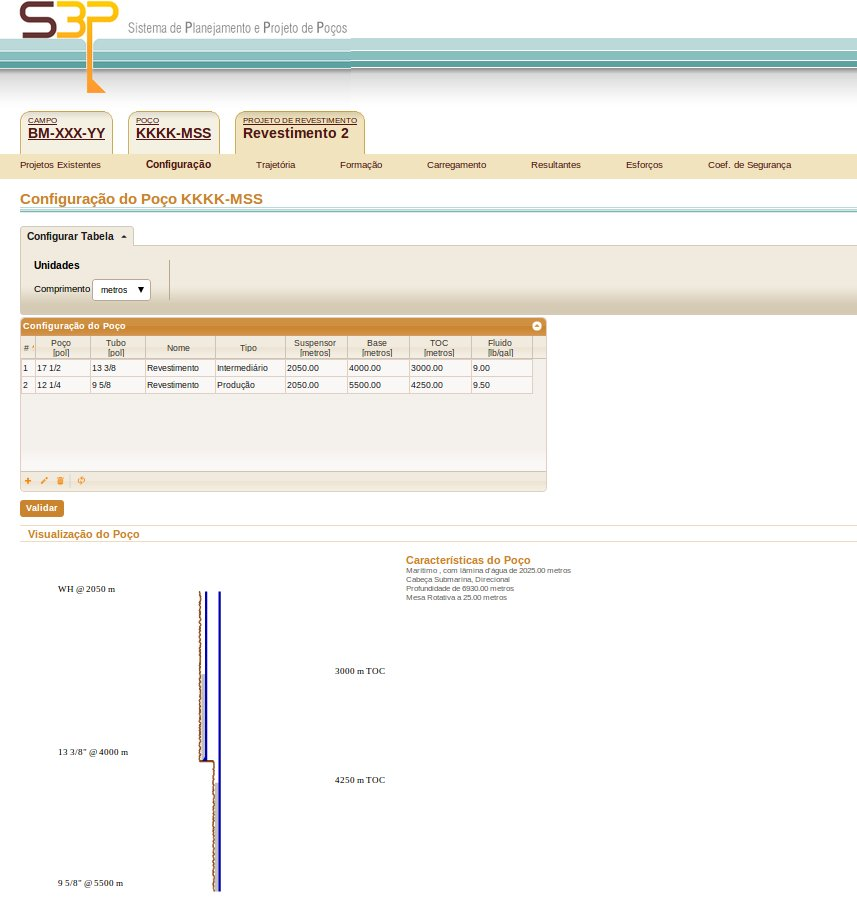
\includegraphics[scale=.5]{./s3p}
\caption{Estrutura de abas do sistema Revestir}
\label{fig:s3p}
\end{figure}

O sistema Revestir foi criado, desde o início, com uma interface WEB projetada para automatizar processos de trabalho que eram antes executadas em papel ou com o auxílio de planilhas. No contexto da visualização de informação, o sistema apresenta como pontos de interesse a criação dinâmica de um infográfico do projeto de poço e o uso de tabelas e gráficos associados. Além disso, abordaremos como o sistema foi feito para orientar o pesquisador ao longo do projeto.

\subsection{Fouling}

O simulador FoulingTR é um sistema desenvolvido pela Petrobras para fazer o acompanhamento da eficiência de baterias de pré-aquecimento (BPA) das unidades de destilação atmosférica, craqueamento catalítico e coqueamento retardado.

Os resultados em texto desse simulador eram armazenados em planilhas muito extensas, que chegavam atingir os limites do software de escritório e tornavam o trabalho muito difícil. A melhor manutenção desses dados, além da demanda de outras funcionalidades para exploração e análise dos dados motivaram a criação de uma interface WEB para o sistema.

O uso de gráficos, mapas georeferenciados e infográficos navegáveis, permitindo um acompanhamento virtual na unidade industrial (refinaria ou plataforma) será abordado neste trabalho.

\subsection{CMIP e Programas de Monitoramento}

A atividade biológica afeta a indústria de petróleo e energia de diversas formas, desde atuante principal, como no caso da produção de biodiesel e outros combustíveis a partir de algas, papel coadjuvante no funcionamento dos processos, como na formação de biofilmes em equipamentos, a até mesmo ser possível ameaça ecológica a ser evitada, com no  caso da contaminação por água de lastro de navios vindos de outros ecossistemas.

A Coleção de Microrganismos da Indústria do Petróleo (CMIP) tem como objetivo preservar, manter e distribuir aos grupos de pesquisa do CENPES/Petrobras, culturas de microrganismos viáveis para utilização nos diversos campos da pesquisa biotecnológica aplicados a exploração, produção de petróleo e energias renováveis. Essa coleção é gerida com o auxilio de um sistema WEB para cadastro e consulta de microrganismos. 

Em alguns casos, é realizado o monitoramento de microrganismos ao longo dos processos industriais. Nos programas de monitoramento de algas e de água de lastro, a aplicação de visão computacional em algumas dessas imagens produz uma quantidade muito grande de regiões de interesse (ROIs).

Processo semelhante também está sendo usado para o acompanhamento do ciclo de vida de colêmbolos para avaliar a toxicidade de algumas amostras de solo.

\begin{figure}[!ht]
\centering
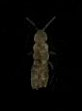
\includegraphics[scale=1]{./image-diff13-12-crop}
\caption[]{Colêmbolo identificado por visão computacional}
\label{fig:image-diff13-12-crop}
\end{figure}

Neste trabalho abordaremos as soluções utilizadas para filtragem, análise e visualização dessas informações.

\subsection{ARGUS}

O sistema WEB ARGUS é uma ferramenta padronizada e personalizada para a análise, diagnóstico e acompanhamento contínuo das unidades de refino.

Os dados manipulados por este sistema são fornecidos por sensores nas instalações industriais. Eles podem ser visualizados como tabelas e gráficos interativos.

As soluções utilizadas para criação e manuseio desses gráficos e tabelas serão abordadas neste estudo.

\subsection{SAGAS}

O sistema SAGAS (Solução Analítica do Gás) é um simulador voltado para compreensão do comportamento de poços e reservatórios. Ele modela o fluxo de fluidos compressíveis em meio poroso, utilizando uma solução derivada do método de Green. \cite{145468-PA}

Os resultados desse simulador são fornecidos em formato texto e precisavam ser transportados para planilhas para análise através de gráficos. Esse proceso era trabalhoso e por particularidades dos dados nem sempre produzia um entendimento adequado dos resultados, o que acabou demandando a criação de uma interface WEB para o mesmo.

Um ponto de destaque nesse estudo é a implementação da interface deste sistema. O uso de gráficos em escalas diferentes, inclusive no mesmo conjunto de dados para se obter a visualização adequada serão abordados.

\subsection{STRITA}

O sistema STRITA (Análise de testes de injetividade em Reservatórios Estratificados) é um simulador de um processo de completação de poços, que modela testes de injeção de água e analisa o fluxo bifásico em um reservatório de óleo com múltiplas zonas de produção (multicamadas).\cite{142746-MS}

Os resultados desse simulador são textos extensos e de difícil interpretação, mesmo depois da exportação dos mesmos para planilha e com a plotagem de gráficos. Essa dificuldade motivou a criação de uma interface WEB para o sistema.

O uso de uma animação feita a partir de gráficos nessa interface e como ela permite a anotação de pontos específicos para exibição estática, será abordado neste trabalho.

\section{Revisão de Literatura}

\subsection{Percepção} 
\label{sec:quant}

A comunicação almejada pela visualização de informação é feita pelo meio visual, canal de recepção de informação ao qual são dedicados 70\% dos receptores de sentido do corpo humano.\cite{few2012show}  O processamento dessa informação é feito em diversas etapas que sumarizam e abstraem a mensagem a ser entendida. Estima-se que apenas 10\% da informação percebida pelos olhos seja transmitida da retina ao cérebro pelo nervo ótico e no cérebro ela é primeiramente processada rapidamente em níveis automáticos e inconscientes. \cite{Ward:2010:IDV:1893097}

As informações processadas pelos olhos são enviadas para memória icônica do cérebro pelo nervo óptico e ficam ali por menos de um segundo enquanto uma interpretação extremamente rápida acontece. Esse processamento, automático, inconsciente e limitado apenas a reconhecimento, é chamado de processamento de pré-atenção (pre-attentive). Ele detecta um conjunto limitado de atributos, como cor, posição e forma e tem um papel importante na produção visual - para se destacar um grupo de objetos, é recomendado usar atributos de pré-atenção. \cite{journals/tvcg/HealeyKRMA08}

Porém, muitos desses atributos não permitem ou são limitados em termos de percepção quantitativa, sendo a posição e o comprimento mais adequados. Atributos visuais como cor e tamanho não são compreendidos pelo cérebro como valores absolutos mas como diferenciais dependentes de contexto, podendo causar confusões e até mesmo ilusões de ótica, efeitos que devem ser evitados na produção de comunicação visual.

A informação visual segue da memória icônica para memória de curto prazo, onde o cérebro combina o que considera útil em agrupamentos visuais, em um processo consciente de atenção. O cérebro só consegue interpretar um número pequeno de agrupamentos por vez e que para processar mais grupos, outros precisam ser esquecidos ou movidos para memória de longo prazo. 

Se um gráfico apresentar dez séries de dados utilizando cores ou símbolos diferentes para cada uma delas, é preciso considerar que o leitor vai precisar de várias consultas a legenda do gráfico para compreensão do mesmo.

É importante tentar evitar essa situação e manter a percepção da informação no nível inconsciente, pois isso facilita a leitura e aumenta a chance de que a transmissão da mensagem seja concretizada corretamente. Níveis mais elevados de consciência são recursos limitados que podem não estar disponíveis no momento da leitura da informação. A resposta a essa indisponibilidade pode variar da mera recusa consciente à leitura ou no pior caso, à substituição inconsciente da mensagem por estereótipos e pré-concepções. \cite{baumeister2011willpower}

\subsection{Cores}

A combinação de cores pode passar desapercebida quando é agradável, mas pode ser bastante incômoda quando mal selecionada. As cores utilizadas na visualização devem ter um relacionamento entre si que promova equilíbrio e harmonia visual. \cite{worqx:Online}
As combinações de cores mais utilizadas em geral se relacionam entre si na forma de variações de relacionamentos monocromáticos, complementares ou triádicos em relação ao círculo cromático.
No relacionamento monocromático, as cores apresentam variações de intensidade de luminância do mesmo tom.

\begin{figure}[!ht]
\centering
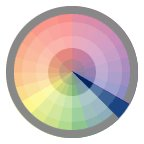
\includegraphics[scale=.7]{./monocromatic_template}
\caption[]{Relacionamento Monocromático}
\label{fig:monocromatic_template}
\end{figure}


No relacionamento complementar, as cores utilizadas se posicionam em extremos opostos no círculo cromático. Essa disposição aumenta o contraste entre as cores, a luminância das mesmas deve ser baixa.

\begin{figure}[!ht]
\centering
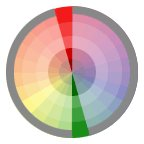
\includegraphics[scale=.7]{./complementary_template}
\caption[]{Relacionamento Complementar}
\label{fig:complementary_template}
\end{figure}

No relacionamento triádico, cores de três tonalidades equidistantes no círculo cromático são selecionadas.
 
Indendente do relacionamento entre as cores escolhidas para o projeto, deve ser evitado o uso de cores totalmente saturadas, pois elas aumentam muito o contraste total da visualização. 

\begin{figure}[!ht]
\centering
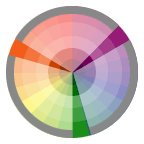
\includegraphics[scale=.7]{./triad_template}
\caption[]{Relacionamento Triádico}
\label{fig:triad_template}
\end{figure}

O contraste deve ser reservado para facilitar a leitura de pontos críticos na visualização, como por exemplo, nas informações em formato de texto, que deve ter pelo menos 80 por cento de contraste.

\subsection{Texto, Tabelas e Gráficos}

O uso de tabelas e gráficos é comum atualmente, mas poucos aprenderam como torná-los eficazes, inclusive porque esses recursos só tiveram sua produção disseminada após a invenção do computador pessoal no final do século 20.

Quando a informação consiste apenas de um ou dois números a linguagem escrita é mais eficaz em termos de comunicação. Uma tabela simples bem projetada, pode fornecer melhor entendimento e mais informação que um gráfico mal feito, apesar de todo apelo e facilidades perceptivas do meio visual. Existe elegância na simplicidade. \cite{few2012show}

A figura \ref{fig:tabgraf1}  mostra uma combinação de tabela e gráficos das últimas 10 temperaturas medidas em um centro de processamento de dados, sendo apenas a última medição relevante. Compare com a figura \ref{fig:quadrotemp}. Além de refletir a disposição geográfica da CPD, as temperaturas críticas passaram a ser marcadas em vermelho.

Para informações quantitativas a mensagem sempre está ligada a alguma coisa relevante sendo medida e esse relacionamento deve ser expresso claramente.

A informação quantitativa pode expressar alguma agregação ou sumarização de um conjunto grande de números. Nesses casos, gráficos são recursos indicados, facilitando bastante a comunicação.

Todas as práticas gerais de projeto orientado para comunicação buscam dois objetivos fundamentais: destacar e organizar os dados.
O destaque adequado aos dados pode ser obtido utilizando o conceito de Edward Tufte, aplicável tanto a gráficos e  tabelas, que consiste em remover elementos desnecessários, evitar o destaque aos elementos visuais estruturais alheios aos dados e se concentrar nos dados. \cite{tufte1983visual}

\begin{figure}
\centering
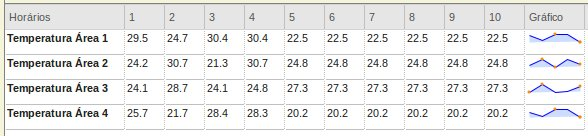
\includegraphics[scale=.5]{./tabgraf1}
\caption{Combinação de tabelas e gráficos}
\label{fig:tabgraf1}
\end{figure}

\begin{figure}
\centering
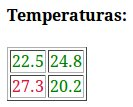
\includegraphics[scale=1]{./quadrotemp}
\caption{Quadro de temperaturas}
\label{fig:quadrotemp}
\end{figure}

Tabelas podem ser usadas sempre que uma relação existir entre valores de conjuntos separados, pois permitem alinhar valores relacionados, se estes forem posicionados na mesma linha ou coluna, facilitando a comparação. Também facilitam a busca de valores individuais e são mais precisas que gráficos.

Gráficos, por sua vez, são mais eficazes quando a mensagem está relacionada ao que é expresso pelo conjunto completo dos dados, como por exemplo, sua tendência no tempo. Ressaltam as exceções e facilitam a visualização de similaridades e diferenças entre conjuntos de dados, pois dão forma a eles.

\subsection{Tabelas} 

No projeto de tabelas, é uma boa prática de visualização usar o mínimo de separadores possível e deixar que a própria estrutura do texto e o espaçamento (espaço em branco) moldem a tabela. Quando o espaço da tabela é muito pequeno, isso pode se tornar inviável e então grades e separadores devem ser usados, mas com cautela.

Esses elementos, além das cores e fontes do texto, podem ser usados para enfatizar a partes importantes dos dados. Ao lidar com dados numéricos em tabelas, é importante levar em conta o alinhamento do texto e a formação numérica (truncagem, notação científica, número de casas decimais, percentuais). Destacar agregações como totais e médias facilita a leitura.

A figura \ref{fig:table2} mostra na parte superior uma tabela que apresenta alguns problemas de visualização. O uso de separadores é visualmente agressivo e a formatação dos campos numéricos à esquerda torna a leitura mais difícil. Saldos negativos não são marcados por cor ou negrito. Além disso, a totalização é apresentada da mesma maneira que as outras linhas, sem distinção.  Abaixo, temos uma sua versão melhorada da mesma informação, que se aproveita da disponibilidade de mais espaço para abrir mão dos separadores e usa cores para dar maior enfâse na agregação e nos saldos negativos.

\begin{figure}[h]
\centering
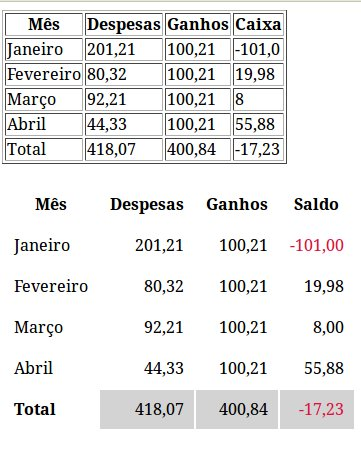
\includegraphics[scale=.5]{./table2}
\caption{}
\label{fig:table2}
\end{figure}

Tabelas são amplamente utilizadas em sitemas científicos. A partir da definição básica de tabela do padrão HTML, muitas adaptações podem ser feitas, desde recursos básicos de visualização, como alternância de cores nas linhas a implementações mais elaboradas, como o uso de fontes coloridas para destaque de erros e pontos de atenção nos dados. 

Dentre os recursos disponíveis estão a possibilidade de reordenação das tabelas a partir de alguma coluna selecionada ou para tabelas maiores uma barra de rolagem mantendo o cabeçalho fixo, a edição de dados e o autocompletar de campos.

A possibilidade de edição dos dados por vezes torna a programação de tabelas uma tarefa complexa. Um pequeno conjunto de regras de validação mal especificadas pode rapidamente tornar a implementação impossível por incoerência ou exponencialmente complexa e inviável para tabelas com maior quantidade de dados. 

\subsection{Gráficos}

Diferentes tipos de relacionamentos quantitativos demandam diferentes formas de gráficos. Dentre as formas mais comuns temos os gráficos de pontos, linhas, barras e de área.

O gráfico de área mais conhecido é o gráfico de pizza que causa problemas de percepção e tem seu uso não recomendado. Quando for crucial manter em foco a visão das partes em relação ao todo, gráficos de pilha (stacked bar) são uma alternativa. Figura \ref{fig:pizzavsbarras}

\begin{figure}[!ht]
\centering
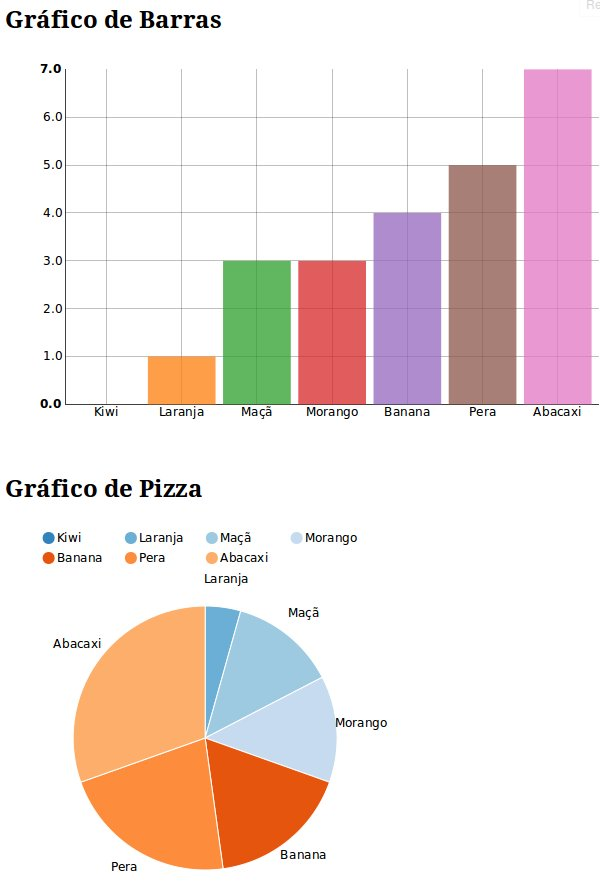
\includegraphics[scale=.3]{./pizzavsbarras}
\caption{Grafico de barras apresentando melhor os mesmos dados que um gráfico de pizza.}
\label{fig:pizzavsbarras}
\end{figure}

Gráficos devem atender o objetivo de corretamente fazer a correspondência das quantidades com a escala visual. Este objetivo, por si mesmo conflita com o uso de efeitos 3D estéticos em gráficos. 
Os atributos de comprimento de linha e posicionamento 2D fornecem boa percepção visual das quantidades e devem ser usados nos gráficos. Outros atributos, como cor e área não permitem a percepção adequada de quantidades.
Para evitar erros de interpretação, os gráficos devem preferencialmente usar a mesma escala entre os eixos e essas escalas devem começar do zero. Quando isso não for adequado para visualização dos dados, deve-se alertar sobre a diferença. As marcas nos eixos (ticagem) deve ser consistentes, sem ausências mesmo em intervalos que não contenham dados.
A figura \ref{fig:anscombe} mostra como uma visualização pode mudar alterando um único elemento de um gráfico.

Os valores podem ser representados nos gráficos através de pontos, barras ou linhas. 
Quando pontos são usados para representar as quantidades, eles devem ser visualmente distintos.  Símbolos e cores diferentes ajudam a manter essa distinção. Rótulos, legendas e marcas de ticagem facilitam a interpretação correta dos dados e por isso fornecem informação crucial, mas devem ser visualmente menos destacados que os valores. A quantidade de marcas de ticagem deve ser suficiente para determinar os valores dos dados dispostos entre elas. Marcas de ticagem menores normalmente sugerem um nível de precisão que o gráfico não possui e só são úteis em escalas logarítmicas.

\subsection{Quarteto de Anscombe }

Quarteto de Anscombe é o nome dado a quatro conjuntos de dados que aparentam ser idênticos quando descritos por certas técnicas de estatística descritiva (como a média e a variância), mas que são muito distintos quando exibidos graficamente. Ele leva o nome do estatístico F.J. Anscombe que o publicou pela primeira vez em 1973 , com o objetivo de demonstrar tanto a importância de se visualizar os dados antes de analisá-los quanto o efeito dos outliers nas propriedades estatísticas. \cite{1973}

\begin{figure}[!ht]
\centering
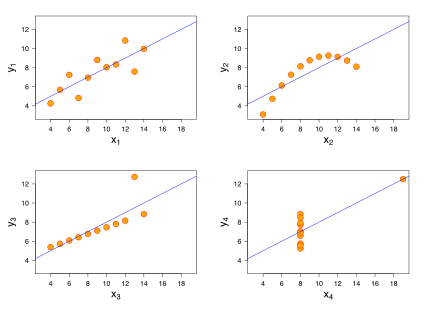
\includegraphics[scale=.7]{./anscombe}
\caption[Quarteto de Anscombe]{Quarteto de Anscombe}
\label{fig:anscombe}
\end{figure}

\subsection{Séries Temporais}

É o tipo de gráfico mais utilizado mas detalhes como diferenças de formato de hora e data, a internacionalização e a variabilidade intervalo de tempo a ser mostrado tornam complexa a implementação de programas computacionais dedicados a produção desses gráficos. \cite{tufte1983visual}

\subsection{Animações}

A criação de animações atualmente é bastante facilitada tanto pelas tecnologias da WEB quanto pela vasta literatura conceitual disponível sobre como produzi-las.

Animações podem ser uma técnica poderosa quando usadas apropriadamente ou muito ruim quando mal utilizadas. Podem aumentar o apelo visual, mas podem dificultar a exploração visual.

Podemos entender a animação como uma série de mudanças visuais entre os quadros. É fácil entender o que aconteceu quando o número de mudanças é pequeno e a animação fica mais complexa conforme as mudanças aumentam.

Objetos se movendo na mesma direção e velocidade serão percebidos como um único grupo. Objetos com suas próprias trajetórias se destacarão visualmente como separados. É difícil acompanhar mais de quatro ou cinco objetos separadamente. Os olhos passam a seguir apenas alguns e tratam os outros como ruído \cite{Cavanagh2005349}.

A animação é bastante utilizada em visualização científica por partir de dados tridimensionais e ser muito difícil mostrar os processos ao longo do tempo de outra forma.

Em contraste, a visualização de informação normalmente lida com espaços de dados abstratos onde as dimensões não correspondem àquelas do mundo real. Por isso, existe comparativamente muito menos exemplos de animações publicadas na comunidade de visualização de informação.

Em mais de cem estudos de visualização e animação, o uso de animação não apresentou melhor resultado quando comparado ao uso de diagramas estáticos. Em um estudo de visualização de algoritmos, as animações se mostraram eficientes quando permitiam que o funcionamento dos algoritmos fosse manipulado e refletiam essas alterações. Quando assistidas passivamente as animações não se mostraram mais eficientes que outros métodos. \cite{steele2010beautiful}

A visualização GapMinder do Hans Rosling é um caso de sucesso, mas apresenta mais informação que os estudos de percepção demonstram ser possível processar. A apresentação guiada de Rosling parece ser crucial para o sucesso da visualização. 

Estudos no Microsoft Research (MSR) mostraram que a animação é uma forma mais lenta e menos precisa de fornecer informação. Para explorar os dados por conta própria, os usuários precisam reexibir a animação várias vezes para verificar algum fato. Os usuários claramente desejam ter a capacidade de controlar a animação no tempo e isso pode torná-la menos eficiente que uma série de imagens estáticas, pois estas últimas permitem que se vá diretamente para a parte que se quer ver.

No entanto, animações são emocionalmente poderosas e mais envolventes. No contexto de apresentação, os dados e a mensagem já são conhecidas pelo apresentador e o público somente assiste. A animação é apresentada diretamente, sem muitas voltas, ao contrário do que faria alguém explorando os dados. Nesse contexto, a animação é recomendada.

\subsection{Mapas}

O tamanho do mapa e como ele acomoda as informações que devem ser mostradas é um fator importante, mas não tão relevante quanto a forma como os dados são apresentados. \cite{steele2010beautiful}

A geografia é o ponto de partida para o projeto de mapas e parte da experiência de quem vai usá-los. Ela precisa ser estilizada e simplificada, mas os relacionamentos dos pontos de referência devem ser preservados.

Além da geografia, as linhas devem denotar os caminhos a serem seguidos. Mais do que meramente serem usadas separadamente para facilitar a distinção das linhas, as cores podem ser organizadas em espectro para fornecer mais semântica ao mapa. O uso de cores é importante para tornar o mapa mais vasculhável, além de apenas mais legível.

Mapas podem envolver questões emocionais. Algumas cores devem ser preservadas, como o azul representando água. Da mesma forma, representar elementos marcantes por desenhos de suas formas tem mais apelo que rótulos em texto com seus nomes.

O texto também pode ser separado em tons de cinza, guardando o preto para as informações mais relevantes. Bem organizado, o mapa fornece camadas de informação sem comprometer sua clareza e funcionalidade.


\section{Visualização de Informações nos Sistemas} 

\subsection{Revestir}

O sistema Revestir automatizou cálculos e etapas de projeto de poços que eram feitas em planilhas e outros softwares específicos. Esse processo de trabalho não unificado, com regras e metodologias variadas para cada tipo de poço, envolvendo sistemas de unidade diferentes e profissionais que trabalham em unidades distantes gerava o risco de falhas de integração, de esquecimento de etapas e a falhas de comunicação. 

A interface do sistema foi produzida utilizando uma estrutura de abas como metáfora para sistemas como os de "carrinho de compras" dos sites de venda pela internet. Ao final do projeto de um poço, o usuário é avisado pelo sistema sobre qualquer problema e encaminhado para o local onde está o problema, de forma semelhante aos programas de cobrança de imposto de renda.

Fortemente influenciado pela rotina de trabalho, o Revestir foi projetado com as tabelas acima dos gráficos, o que preferimos evitar atualmente. Gráficos são mais usados para análises rápidas de projetos e devem ser apresentandos primeiros. Por outro lado, as planilhas, apesar de serem usadas durante boa parte do tempo, são usadas em atividades mais demoradas como aferição de dados e podem aparecer abaixo. 

Em um projeto típico, mais de 200 regras de negócio são verificadas pelo sistema e apontadas para o usuário em caso de problemas, através variações de cores nas planilhas e mensagens de alerta.

As tabelas foram automatizadas para apontar as falhas mais comuns ao longo do preenchimento, mas durante o desenvolvimento do projeto se mostrou impossível em alguns casos e computacionalmente inviável em outros apontar todas as falhas no mesmo momento. O planejamento de quais regras deveriam ser validadas logo no preenchimento das planilhas e de qual preenchimento poderia ser feito de forma automática consumiu grande parte do tempo de projeto do sistema.

Uma funcionalidade do módulo é a apresentação de um infográfico, que permite ao engenheiro uma rápida visualização estrutural do projeto que está sendo criado. Essa figura é atualizada em tempo real enquanto o módulo está sendo utilizado.

\begin{figure}[!ht]
\centering
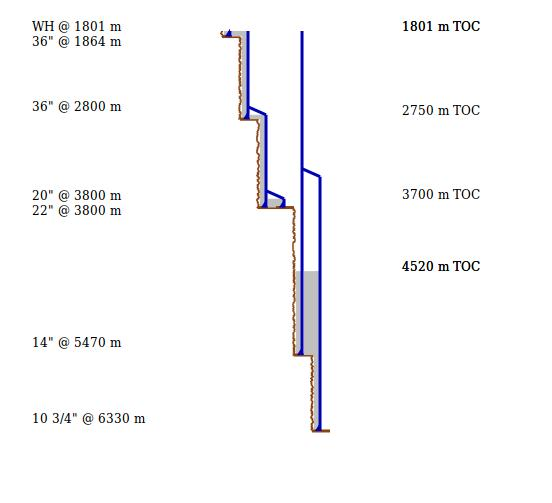
\includegraphics[scale=.5]{./s3p-infografico}
\caption[]{Revestir - Infográfico}
\label{fig:s3p-infografico}
\end{figure}

Nela, cada fase de perfuração é desenhada, na medida do possível, em escala aproximada aos dados reais do projeto, com um tamanho mínimo sendo utilizado no caso de objetos muito pequenos. Como não existe um limite pré-determinado para o tamanho do poço, as dimensões das  fases são normalizadas e desenhadas de acordo com a área disponível para a figura.

Além das fases de revestimento, também é desenhada uma representação da cimentação utilizada em cada fase, a partir do dado Topo de Cimento, inserido no projeto. A posição dessas fases e cimentação é marcada na figura e detalhes como o assentamento e a ligação de revestimentos suspensos (liners) são representados no infográfico.

Para o sistema revestir foi desenvolvida a possibilidade de criação de relatórios para impressão editáveis com a informação dos projetos. 

Como os mesmos princípios de visualização aplicados na interface se aplicam para a informação impressa, não houve grandes mudanças, do ponto de vista da visualização de informação, na passagem desses dados para o formato texto. 

Entretanto, a ausência de interatividade, as necessidades de formatação para impressão em papel diferentes das para apresentação em tela e a necessidade de fornecer edição gerou alguns desafios de implementação que serão descritos mais adiante neste documento.

\subsection{Fouling}

Uma execução do simulador FoulingTR tem como resultados os valores esperados ao longo do tempo relativos a uma série de condições físicas medidas por sensores nas instalações industriais. Em geral, o valor esperado para algumas centenas desses sensores são produzidos, para cada unidade simulada.

\begin{figure}[!ht]
\centering
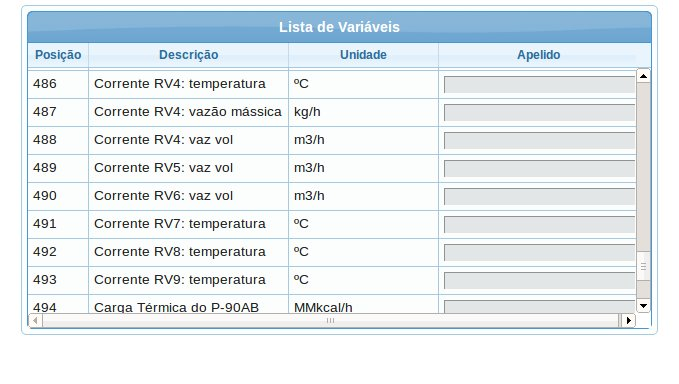
\includegraphics[scale=.7]{./fouling_apelidos}
\caption{Fouling - Variáveis e seus apelidos}
\label{fig:fouling_apelidos}
\end{figure}


Para fins de análise, muitas vezes é preciso comparar valores que possuem forte correlação, mas ordens de grandeza muito díspares, como por exemplo, a temperatura em um equipamento e o seu impacto econômico na unidade. Análises desse tipo são feitas através de gráficos, mas para estes serem úteis é preciso bastante cuidado nos ajustes do número de casas decimais dos dados e nos intervalos dos eixos dos gráficos.

\begin{figure}[!ht]
\centering
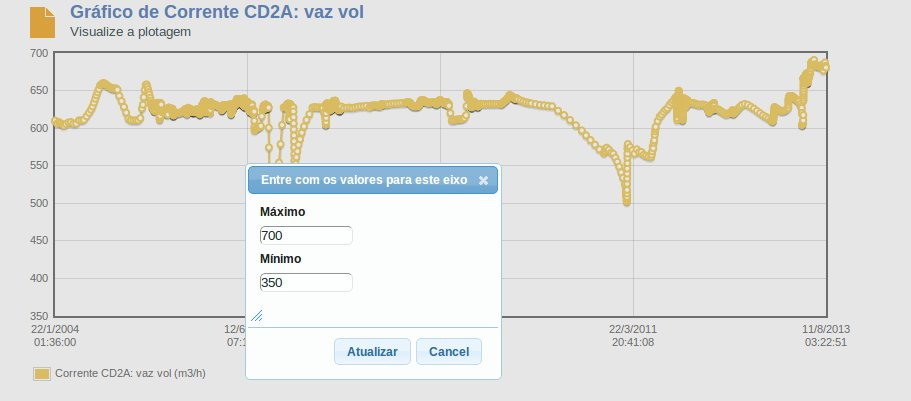
\includegraphics[scale=0.5]{./fouling_intervaloY}
\caption{Fouling - configurando o eixo Y}
\label{fig:fouling_intervaloY}
\end{figure}


Na interface do sistema, esses valores são configuráveis. Além disso, existe também a opção de exibir as séries em eixos sobrepostos o que permite avaliar medidas com ordem de grandeza diferentes no mesmo gráfico. Existe também  um esperado ruído nos dados e as curvas precisam ser suavizadas. Na interface elas são apresentadas com o recurso de  média móvel configurável para suavização.

\begin{figure}[!ht]
\centering
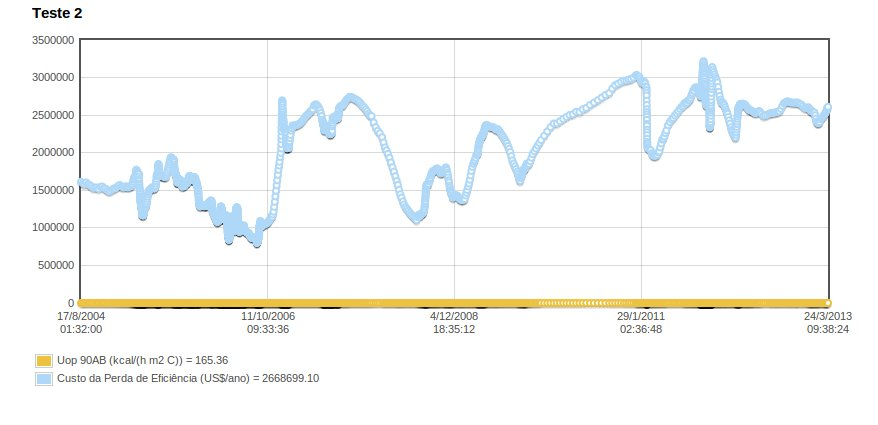
\includegraphics[scale=0.5]{./fouling_sem_multieixo}
\caption{Fouling - Sem múltiplos eixos}
\label{fig:fouling_sem_multieixo}
\end{figure}

\begin{figure}[!ht]
\centering
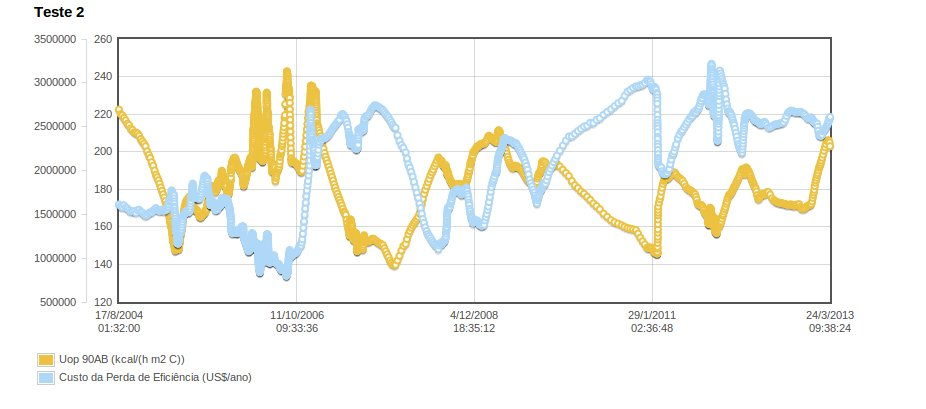
\includegraphics[scale=0.5]{./fouling_com_multieixo}
\caption{Fouling - Com múltiplos eixos}
\label{fig:fouling_com_multieixo}
\end{figure}

\begin{figure}[!ht]
\centering
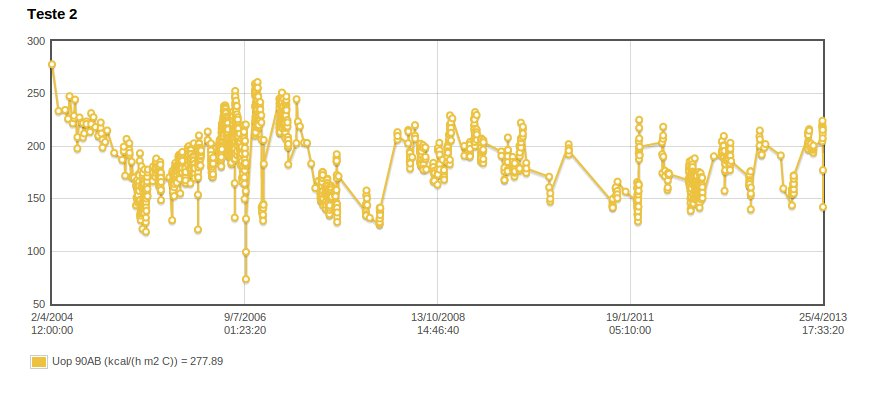
\includegraphics[scale=.5]{./fouling_sem_suavizar}
\caption{Fouling - Sem média móvel}
\label{fig:fouling_sem_suavizar}
\end{figure}

\begin{figure}[!ht]
\centering
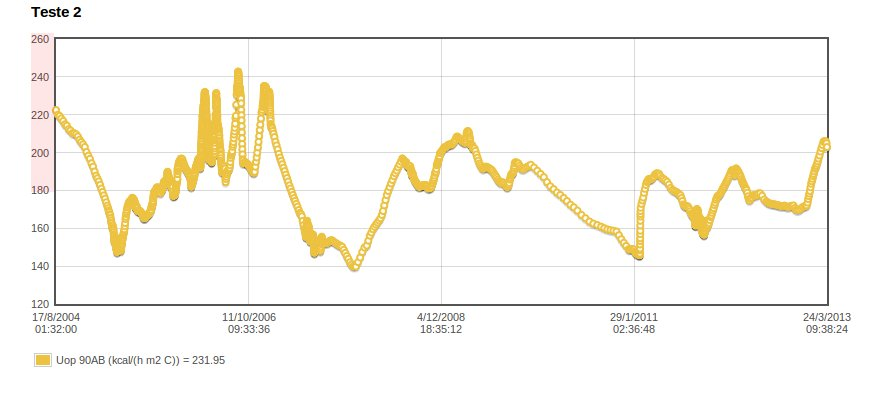
\includegraphics[scale=.5]{./fouling_suavizada}
\caption{Fouling - Com média móvel}
\label{fig:fouling_suavizada}
\end{figure}

Apesar do sistema ser todo voltado para visualização de gráficos, seguindo a filosofia de não aprisionar os dados,a interface tem opções para fornecer arquivos textos com os resultados para todas as medidas em um dado momento e também, em formato de planilha, o conjunto dos dados exibidos em um gráfico. 

Para rápida conferência, os gráficos são iterativos e os valores exatos de cada ponto são exibidos em "tooltips" quando se passa com o mouse por cima deles.

Mesmo assim, a visualização de valores relativos a centenas de medidas, identificadas por nomes nem sempre muito significativos tornava difícil a utilização do sistema, em especial para pessoas de outras unidades ou da administração central. 

As primeira versão da interface tentava mitigar isso com a possibilidade de se configurar nomes alternativos para cada medida, mas isso só resolvia parte do problema.

A solução que adotamos posteriormente para o problema foi a configuração de mapas navegáveis para cada unidade industrial onde o sistema é utilizado. O número de medidas para cada unidade e a demanda de popularizar o sistema nos desencorajou a utilizar qualquer solução que gerasse os mapas automaticamente.

Como se trata de mapas interativos exibidos no computador, usuário é apresentado a uma visão geral da unidade. Cada seção da unidade (ramal) é representada nessa visão geral com um símbolo clicável. Cliques nesses símbolos de ramais ou de outros equipamentos mais complexos conduzem a visões expandidas, que apresentam as medidas correspondentes. Cliques nas medidas levam a visualização de gráficos da mesma e "tooltips" fornecem o nome de cada uma. Além disso, a visualização apresenta um calendário, que também permite a visualização dos dados apresentados no tempo.

\begin{figure}[!ht]
\centering
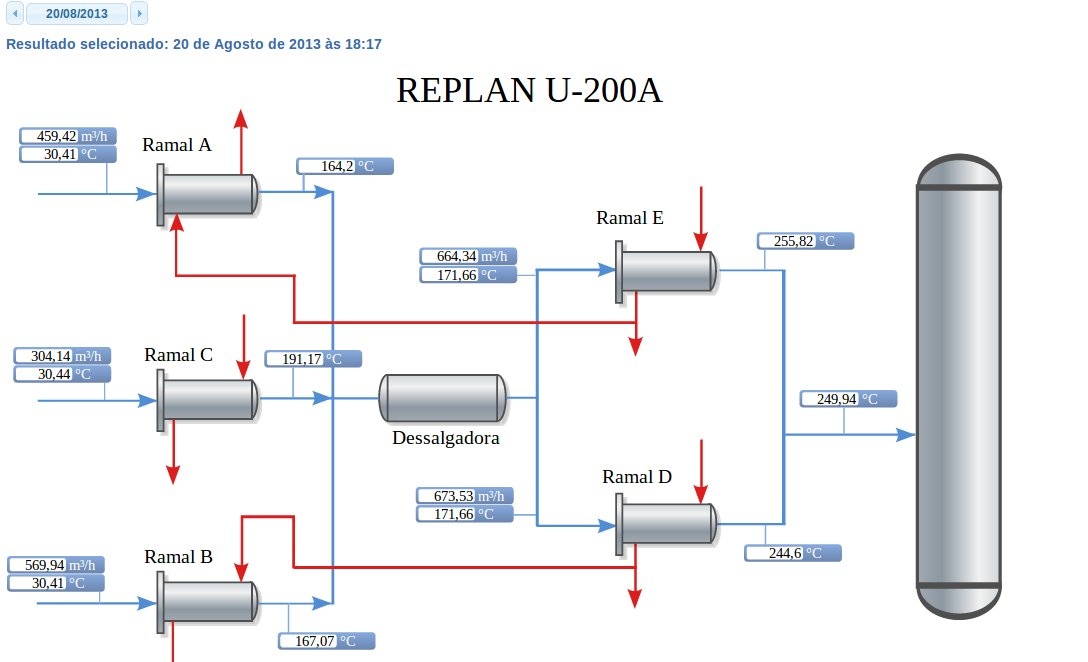
\includegraphics[scale=0.4]{./fouling_diagrama}
\caption{Fouling - diagrama de unidade}
\label{fig:fouling_diagrama}
\end{figure}

Esses mapas seguem vagamente a geografia das unidades. Além disso,  para facilitar a localização dos dados no mapa pelos clientes do sistema, ícones de apelo emocional como o flare e os trocadores foram confeccionados e cuidadosamente posicionados nos mapas.

Por último, para orientar os clientes que possuem acesso a dados de mais de uma unidade ou mais de uma instalação industrial uma estrutura de árvore permite ao cliente navegar para a unidade que quiser em qualquer uma das instalações. Atualmente mais de vinte unidades estão representadas no sistema, com diversas unidades cada.

\begin{figure}[!ht]
\centering
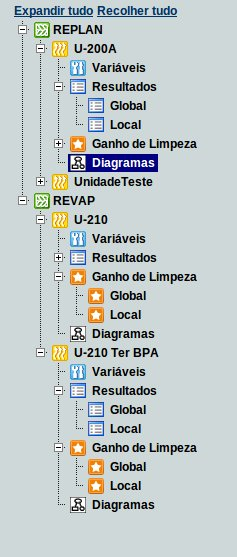
\includegraphics[scale=.5]{./fouling_arvore}
\caption{Fouling - Árvore de navegação}
\label{fig:fouling_arvore}
\end{figure}

\subsection{SAGAS}

O resultado do simulador do sistema SAGAS, fornecido em formato texto são dados que correspondem a funções e suas derivadas. A correta interpretação dos mesmos só pode ser feitas através de gráficos e estes precisam ter seus eixos nas escalas apropriadas para visualização, sendo utilizados escalas lineares, logarítmicas e mistas, em uma configuração muito similar à descrita pelo Quarteto de Anscombe.

\begin{figure}[!ht]
\centering
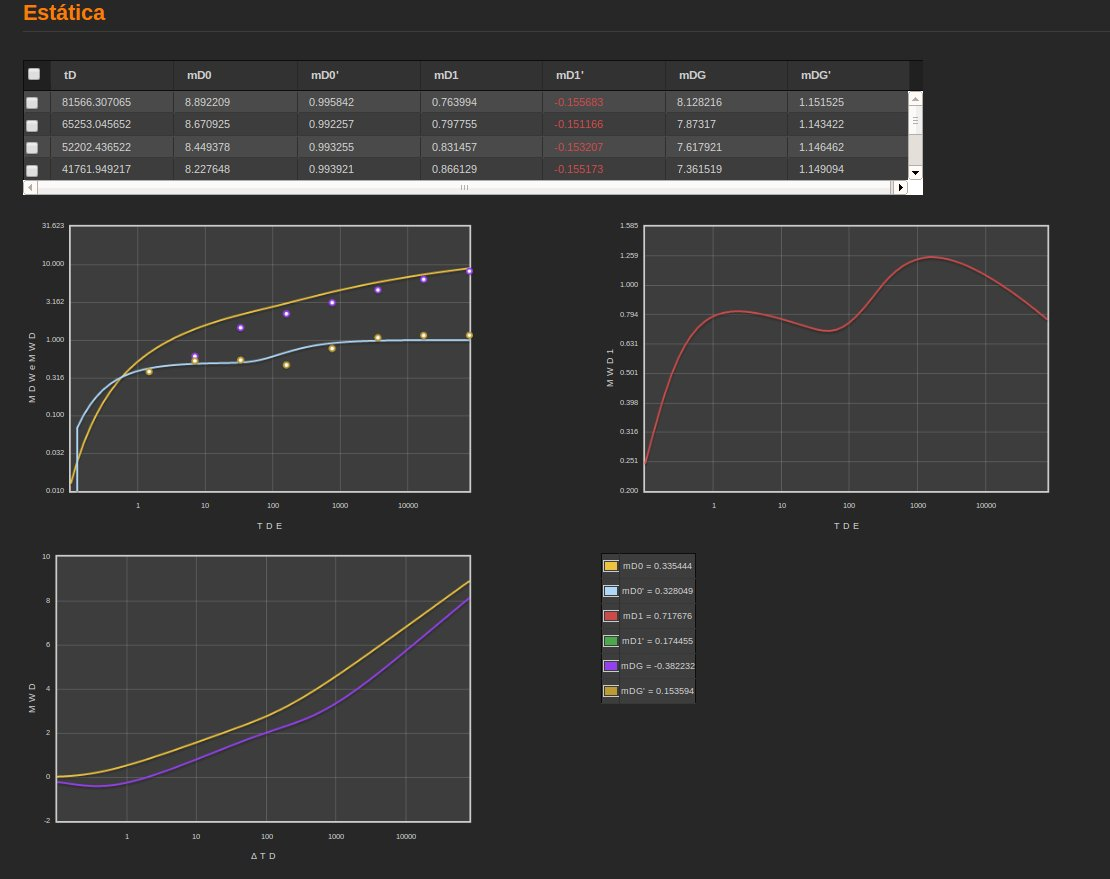
\includegraphics[scale=.3]{./sagas}
\caption{SAGAS - Gráficos com diferentes escalas}
\label{fig:sagas}
\end{figure}


Na interface do sistema SAGAS, a tabela ainda apresentada na parte superior da página, podem ser analisada através de três gráficos iterativos. O primeiro apresenta uma parte dos dados da tabela em uma interpolação de pontos sobreposta por um gráfico de dispersão, com ambos os eixos em escala logarítmica. 

No segundo, apenas o eixo y tem escala logarítmica e o terceiro apresenta os eixos em escala linear. A legenda unificada dos três gráficos apresenta os valores de forma iterativa, atualizados conforme o passar do mouse nos pontos plotados. O conjunto desses valores em cada ponto equivale a uma linha da tabela.

A implementação desses gráficos pode se tornar complicada. No caso do sistema SAGAS, programação adicional teve que ser realizada para exibir os eixos com escala não linear e para unificar a legenda. Além disso, para plotagem dos gráficos de dispersão um algoritmo de amostragem (sampling) teve que ser aplicado. Para as curvas interpoladas, ao contrário foram fornecidas as opções de interpolação linear a cada ponto ou o uso de splines. 
 
\subsection{STRITA}

O simulador do STRITA fornece uma saída de texto muito grande na forma de diversas tabelas. O sistema possui um recurso de visualização que permite a comparação de dados reais com dados simulados, na mesma plotagem.

Os resultados do simulador podem ser analisados através da plotagem de segmentos desses dados, que representam um momento no tempo. Entretanto, o conjunto completo dos resultados realmente modela uma animação do avanço do fluido injetado nas camadas do reservatório. 

Esse avanço varia muito ao longo do tempo, geralmente sendo muito lento no início do teste e aumentando muito no final. Identificar pontos variações nesse avanço é justamente o objetivo do simulador, mas selecionar esses momentos para análise via plotagem a partir dos dados em texto era um problema.

A solução desenvolvida de visualização foi a plotagem de todos os momentos, sobrepostos através de uma barra de rolagem, criando o efeito de uma animação.

\begin{figure}[!ht]
\centering
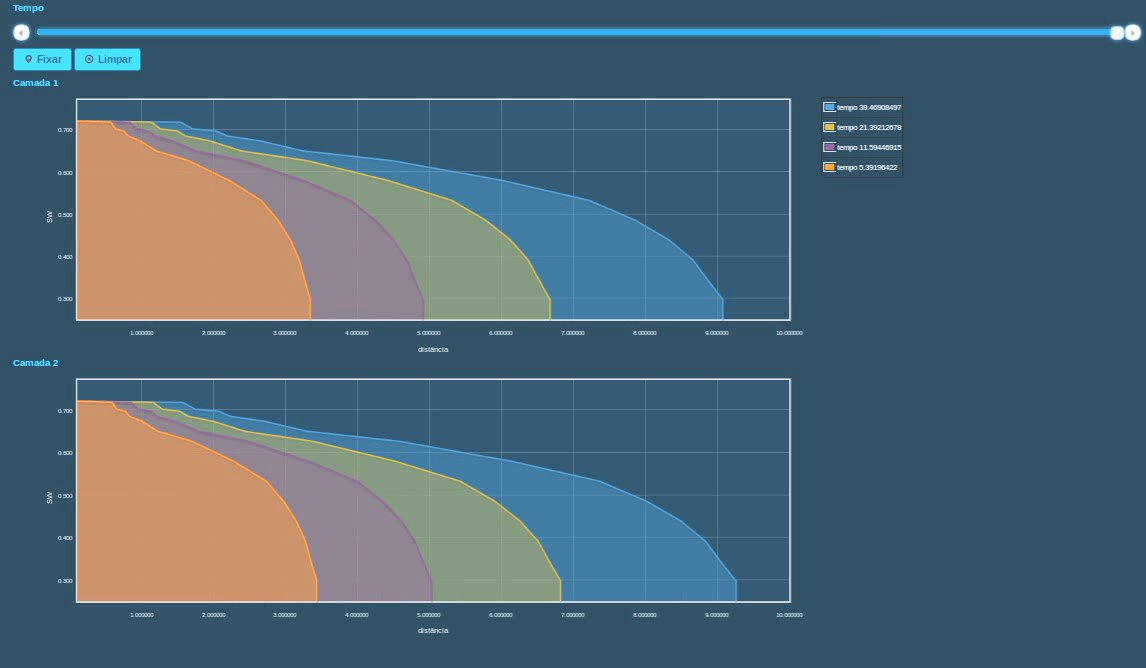
\includegraphics[scale=0.3]{./strita_frentes}
\caption{Strita - Pontos selecionados em duas camadas}
\label{fig:strita_frentes}
\end{figure}

Para que essa animação não atrapalhasse a análise, o código foi bastante otimizado para que a plotagem fosse rápida e que o avanço e recuo no tempo fossem precisos. 

Além disso, foi criada uma funcionalidade permitindo a fixação na animação de momentos no tempo, onde o gráfico do instante selecionado é mantido com uma cor diferente do tom de azul utilizado na animação.

\subsection{ARGUS}

De forma bastante semelhante ao sistema Fouling, uns dos objetivos do sistema ARGUS é fornecer resultados das análises e previsões, conforme simulado pelo núcleo de cálculo, de dados derivados de medições de centenas de sensores da diversas instalações industriais. 

O sistema é utilizado para promover consultas e comparações dessas análises e medidas. O sistema permite a plotagem de diversos tipos de gráficos e a manipulação interativa dos mesmos.

Apesar do contexto dos gráficos ser bastante semelhante ao dos gráficos do sistema FoulingTR, as soluções para manipulação foram bastante distintas. O ARGUS não trabalha com a definição dos intervalos dos eixos, mas disponibiliza recursos de zoom para permitir o ajuste de escalas. 

Para orientar o usuário nesse processo, uma figura pequena com a imagem do gráfico completo, com a seção que está sendo exibida em destaque é mostrada. Um botão para restaurar a configuração original também foi criado.

\begin{figure}[!ht]
\centering
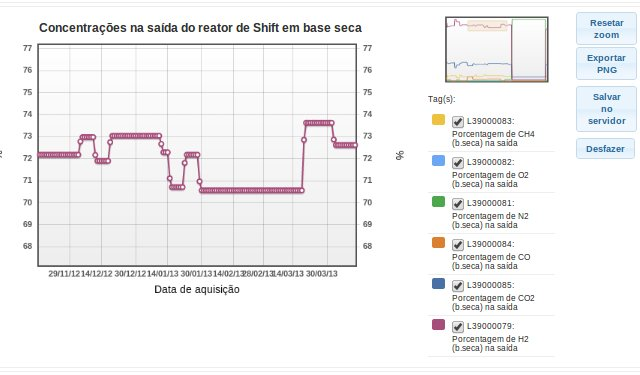
\includegraphics[scale=.7]{./argus_zoom}
\caption{Argus - Zoom}
\label{fig:argus_zoom}
\end{figure}


A funcionalidade de exibição de gráficos com múltiplas escalas nos eixos também não foi implementada e o sistema permite apenas o uso de no máximo duas escalas. Para promover a comparação de variáveis com grandezas muito diferentes o projeto do sistema optou pela exibição na mesma tela de vários gráficos, integrados por um recurso interativo de "crosshair".

\begin{figure}[!ht]
\centering
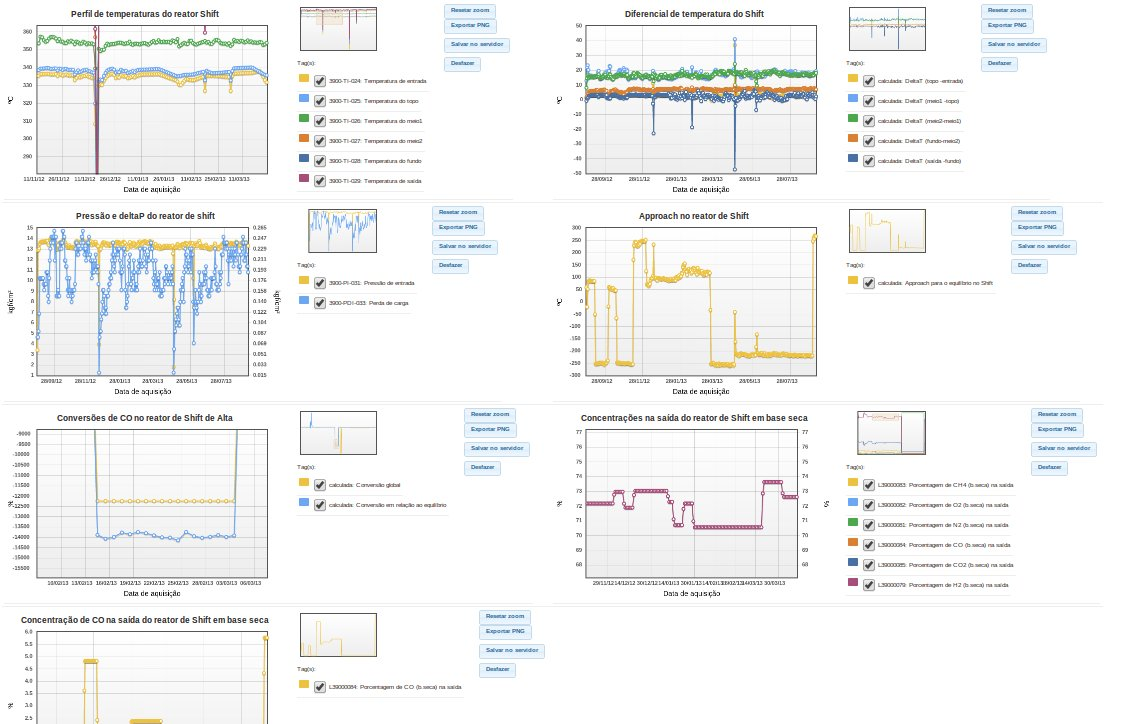
\includegraphics[scale=.4]{./argus_multigraficos}
\caption{Argus - Visualizando múltiplos gráficos}
\label{fig:argus_multigraficos}
\end{figure}

\begin{figure}[!ht]
\centering
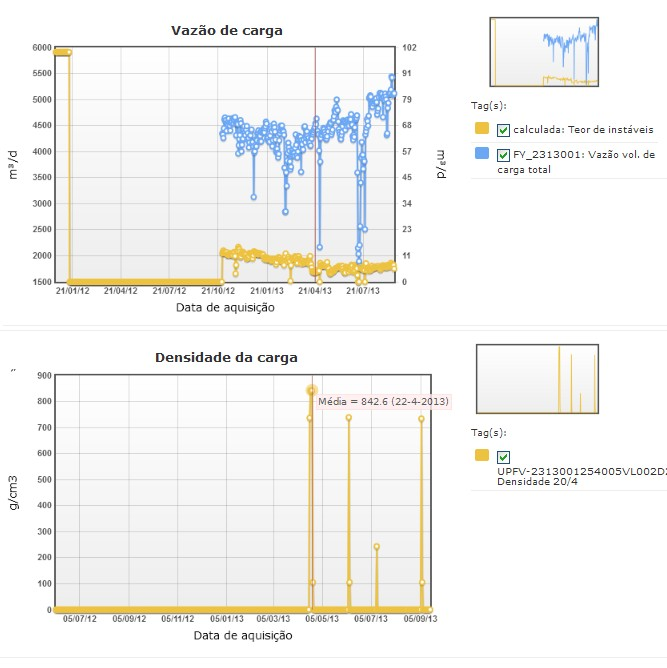
\includegraphics[scale=.4]{./crosshair}
\caption{Argus - Uso do "crosshair"}
\label{fig:crosshair}
\end{figure}


Ao contrário do sistema Fouling, neste sistema também não foi implementada nenhuma suavização dos dados. Entretanto, foi desenvolvida uma funcionalidade para exibir curvas de tendências nos gráficos e um recurso interativo que permite a eliminação de pontos atípicos com um clique do mouse.

\begin{figure}[!ht]
\centering
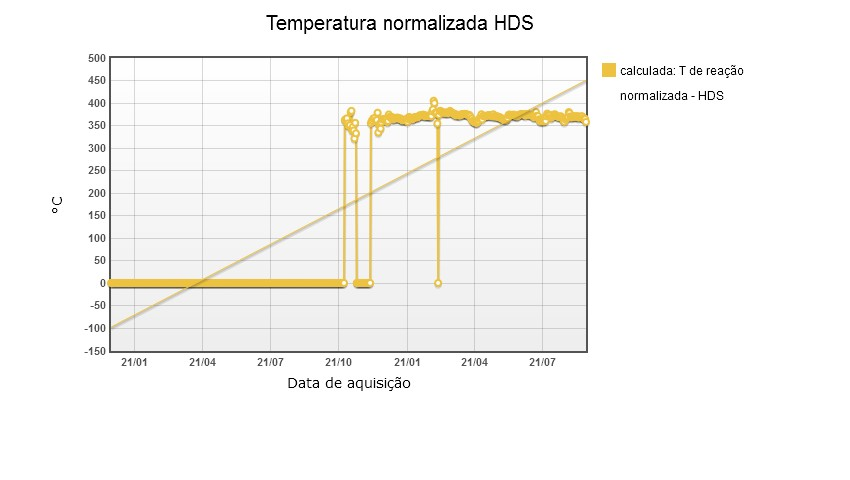
\includegraphics[scale=.4]{./argus_curva_tendencia}
\caption{Argus - Curva de tendência}
\label{fig:argus_curva_tendencia}
\end{figure}

Atendendo a filosofia de não aprisionar os dados, os gráficos e consultas podem ser exportados em formatos de imagem e planilha.

Além disso, o sistema permite a criação de relatórios a partir de uma convenção de códigos. O relatório é editado normalmente pelo usuário em um editor WYSIWYG, no caso o TineMCE. \cite{tinemce:Online} No local onde se deseja um gráfico ou uma tabela, o cliente utiliza um código convencionado para determinar isso.

\begin{figure}[!ht]
\centering
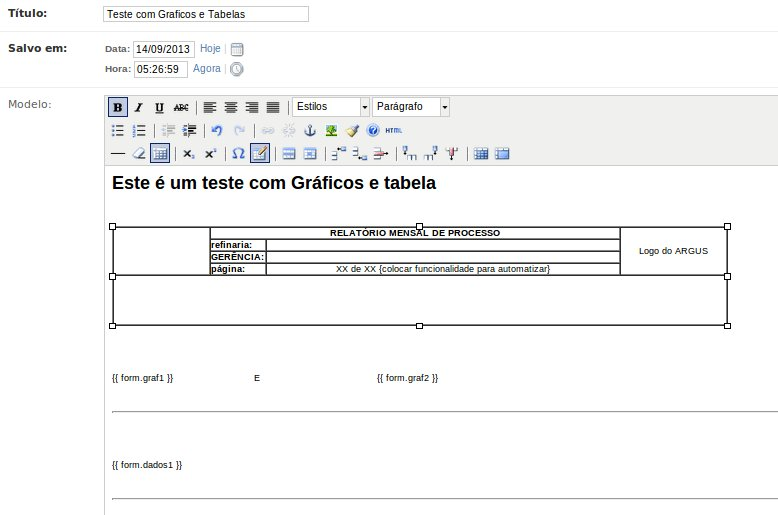
\includegraphics[scale=.5]{./argus_criando_relatorio}
\caption{Argus - Criando o Relatório}
\label{fig:argus_criando_relatorio}
\end{figure}

Esse código é posteriormente substituído por caixas de lista, onde o cliente pode então determinar qual gráfico ou resultado deve aparecer ali. Na etapa final, de pré-visualização do relatório que será impresso, o cliente pode então ver seu relatório completo. Todas as etapas de edição estão reunidas na mesma tela do sistema.

\begin{figure}[!ht]
\centering
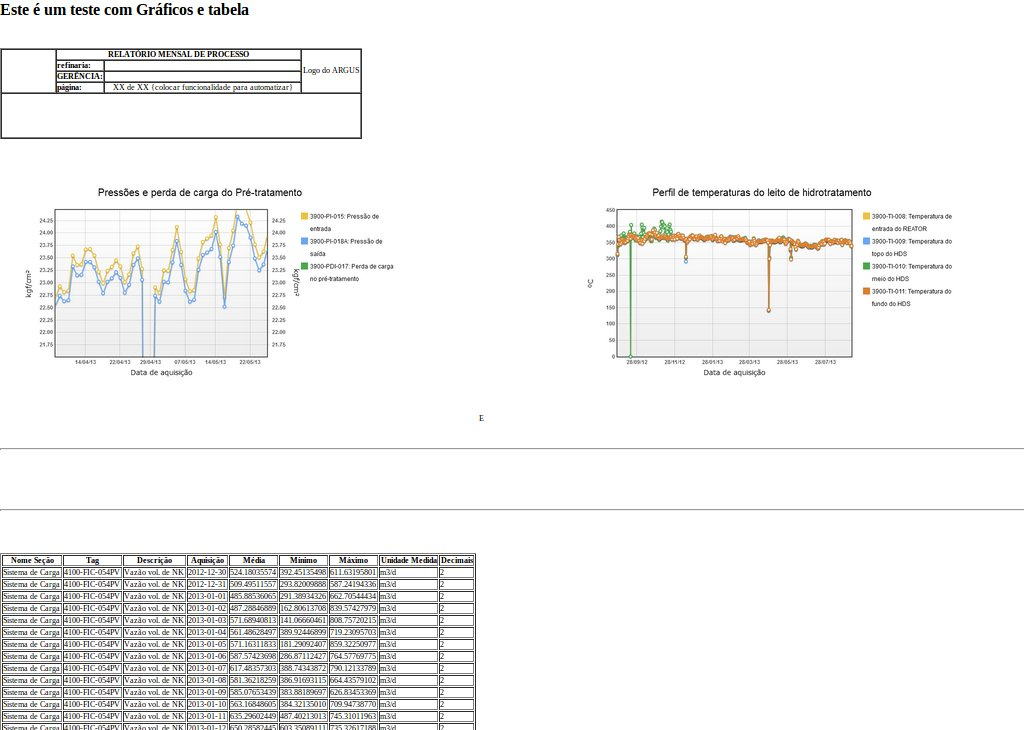
\includegraphics[scale=.5]{./argus_relatorio_criado}
\caption{Argus - Relatório Criado}
\label{fig:argus_relatorio_criado}
\end{figure}

\clearpage{}

\subsection{CMIP} 

Atualmente o sistema de controle da Coleção de Microrganismos da Indústria do Petróleo (CMIP) apresenta fotografias do aspecto microscópico e macroscópico dos organismos para facilitar a identificação dos mesmos.

Para o monitoramento de algas e de análise de água de lastro, foram desenvolvidas ferramentas que controlam a análise da amostra, realizam o reconhecimento via visão computacional e produzem o laudo em planilha. 

Esse reconhecimento não é perfeito e gera um grande número de regiões de interesse (ROIs) que não são o objetivo da análise. Essas ROIs são descartadas de acordo com algumas heurísticas pré-definidas, que levam em conta a cor média da região, a esfericidade, a área, entre outras características levantadas pelo processo de reconhecimento. 

Parte desse processo é manual e, para validação desses resultados, foi desenvolvida uma ferramenta de visualização que destaca o contorno da região identificada na imagem original e outra que concatena todas as regiões identificadas em uma única imagem.

\begin{figure}[!ht]
\centering
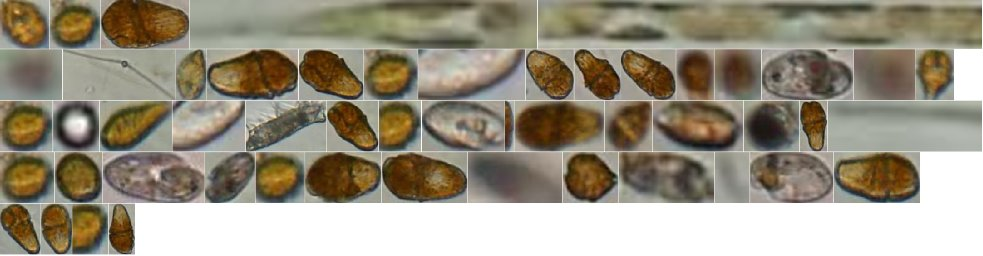
\includegraphics[scale=.35]{./bio_concat}
\caption{Concatenação de regiões identificadas}
\label{fig:bio_concat}
\end{figure}

Em processo semelhante, para monitorar o ciclo de vida dos colêmbolos, utilizamos a diferença de imagens para detectar movimento.

\begin{figure}[!ht]
\centering
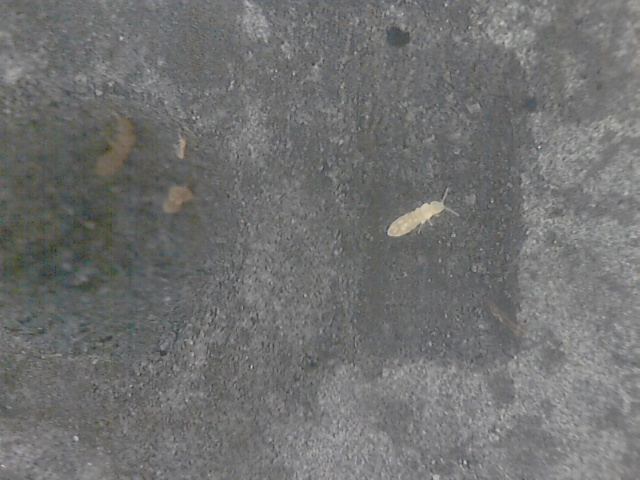
\includegraphics[scale=.25]{./imagedani2-12}
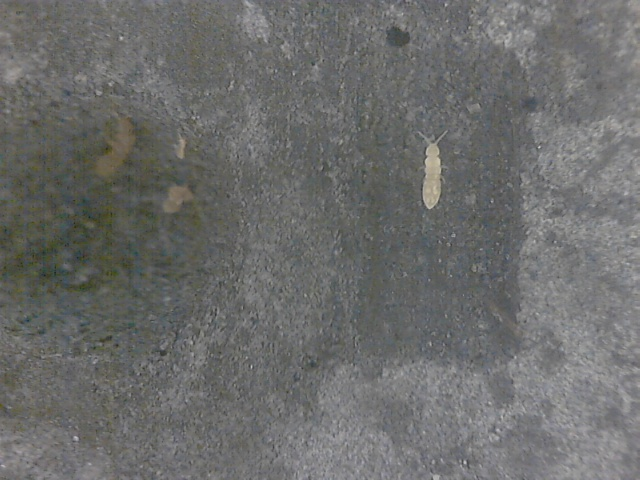
\includegraphics[scale=.25]{./imagedani2-13}
\caption{Sequência de imagens mostrando movimento}
\label{fig:movimento}
\end{figure}

\begin{figure}[!ht]
\centering
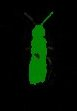
\includegraphics[scale=1]{./image-diff-recog-crop}
\caption{Região de interesse destacada}
\label{fig:roi}
\end{figure}


No momento, estamos integrando essas ferramentas em um modelo de código e documento integrado, utilizando a tecnologia Ipython notebook. \cite{perez:Online}
 
\clearpage{}

\section{Tecnologias}

\subsection{Plotagens em Flot}

Nos sistemas descritos nesse trabalho, as soluções de plotagem foram construídas com a biblioteca Flot. \cite{Flot:Online} 

Ela tem a vantagem de ser uma solução em linguagem javascript, o que permite  permite a produção com gráficos com bastante interatividade dentro do navegador WEB. Outra vantagem de executar o código no navegador é que isso distribui o tempo de processamento nos computadores onde será feita a visualização, evitando a sobrecarga dos servidores.

A biblioteca possui limitações em comparação com a biblioteca python Matplotlib \cite{matplotlib:Online}, que seria nossa opção caso os sistemas não fossem WEB. Por exemplo, as plotagens em escala logarítmica usadas nos sistemas tiveram que ser desenvolvidas internamente. Outras funcionalidades da biblioteca tiveram que ser extendidas para se adequar ao sistema Fouling. O algoritmo que controla a marcação nos eixos (tick marks) teve que ser refeito.

Funcionalidades como a exibição de legendas e marcação de valores de acordo com o movimento do mouse, bem como o destaque de qual eixo estava controlando cada ponto selecionado também tiveram que ser programados. 

Como a API da biblioteca está longe de ser completa, em muitas vezes tivemos que recorrer ao código fonte para fazer essas adaptações. No entanto, a biblioteca se mostrou bastante adaptável, fornecendo acesso aos eventos e permitindo a configuração de tudo foi necessário.

Essa flexibilidade foi fundamental para criação da plotagem animada feita para o Strita. A alternativa considerada antes seria gerar filmes no servidor, o que comprometeria totalmente a usabilidade da ferramenta. 

O resultado, deixando o servidor encarregado somente da seleção dos dados e produzindo toda a exibição da animação no cliente WEB foi muito rápido, o que viabilizou a solução como ferramenta de análise.

\subsection{Mapas e Infográficos em SVG}

Scalable Vector Graphics (SVG) \cite{SVG:Online} é um formato de imagem vetorial 2D baseado em XML com especificação aberta desenvolvida pelo  World Wide WEB Consortium (W3C). Esse formato foi apresenta diversas características que o tornam desejável para o contexto de visualização de informação. Dentre elas:

- É um formato de imagem vetorial, podendo se adequar a qualquer necessidade de tela e de resolução no momento da exibição. 

- É um formato de texto, podendo ser processado programaticamente após sua produção.

- Permite interatividade e suporta animações.

- Pode ser exibido em navegadores WEB.

- Suporta navegação por hyperlinks.

- É programável em linguagem JavaScript.

- Possui ferramentas de edição poderosas e livres, como o software Inkscape ou o SVG Edit.

- Pode ser totalmente processado no servidor WEB e ainda prover interatividade no navegador.

As imagens em arquivos SVG podem ser geradas a partir de softwares de edição manual como o Inkscape ou a partir de bibliotecas de software como o GraphViz, Matplotlib ou Pygal. O ajuste e extensão de funcionalidades desses arquivos é bastante facilitado pelo fato do formato SVG ser meramente um formato de texto. As transformações podem ser realizadas a partir de substituições de string e do uso de expressões regulares. 

A experiência com o Fouling nos serviu de referência para recomendar que o formato SVG para criação de mapas georeferenciados.

Entretanto, a criação manual de mapas e infográficos é trabalhosa e pode demandar mais tempo e recursos que o disponível para o projeto. Nesses casos, a criação de mapas e diagramas automaticamente é possível e para isso podemos utilizar o software Graphviz. \cite{graphviz:Online} Com ele é possível gerar diagramas em formato SVG que podem ser perfeitamente integrados ao processo. 

Quando mapas mais elaborados são necessários, como no sistema Fouling, também utilizamos o formato SVG, mas nesse caso os arquivos com os mapas das unidades de refinaria foram desenhados no Inkscape e nos lugares adequados, foram colocadas palavras chaves predefinidas para indicar qual variável de medição deveria ser apresentada nessas posições.

Com o uso de expressões regulares, foi possível determinar rapidamente quais variáveis de medição deveriam ser usadas. A posição correta foi obtida automaticamente, meramente substituindo a palavra chave (já posicionada corretamente) pela variável de medição correspondente. O mesmo processo foi usado para inserção de gráficos e tabelas no sistema ARGUS.

No sistema Fouling, o software Inkscape foi utilizado para edição das figuras em SVG e uma extensão foi desenvolvida para ele. 

No sistema Revestir A biblioteca originalmente usada para gerar a imagem no formato SVG foi a pySVG \cite{pysvg:Online}. Ela teve sua última atualização em 2010 e se mostrou limitada, ao não permitir especificar a espessura das linhas a serem plotadas. 

Após uma pesquisa, foi escolhida a biblioteca svgwrite \cite{svgwrite:Online}, mais atualizada e bem documentada. Mudar de biblioteca não foi muito difícil, bastou a alteração de alguns comandos. Com a nova biblioteca, foi possível especificar o tamanho da espessura da linha, o que simplificou um pouco o código.  


\subsection{Tabelas com Slickgrid e jqGrid}

As tabelas utilizadas no sistemas Revestir, SAGAS, STRITA, Fouling e SAUR foram criadas com as tecnologias Slickgrid e jqGrid. \cite{SlickGrid:Online} \cite{jqGrid:Online}

Nos sistemas, essas tabelas foram configuradas para facilitar o trabalho dos clientes, fornecer informações relevantes e evitar erros. 

As tabelas foram configuradas para discretamente alternar a cor de fundo a cada linha, para facilitar a visualização. Além disso, as cores das fontes são utilizadas para destacar erros e incoerências. 

Alguns campos foram configurados para exibir caixas de escolha, para evitar erros de digitação e orientar o cliente nos valores possíveis. Em alguns casos, uma caixa de diálogo é exibida para facilitar ao cliente a escolha dos valores de uma célula.

Nos sistemas SAGAS e STRITA, as tabelas possuem alguns recursos de integração com os gráficos que exibem seus valores. Pontos escolhidos a partir da tabela podem ser excluídos dos gráficos e a linha na tabela referente a cada ponto no gráfico é mostrada conforme o posicionamento do mouse.

\subsection{Documentação com Ipython Notebook}

Atualmente a documentação do sistema STRITA e toda a integração das ferramentas de análise de algas e água de lastro está sendo produzida utilizando-se o ipython notebook. \cite{perez:Online}

Sua capacidade de integrar a execução de código python com a criação de documentos com formatações diversas como markdown, html, LaTex e a sua capacidade de exibir imagens e vídeos tem se mostrado muito útil.

Recentemente, nosso grupo reeditou o livro "Python Para Desenvolvedores" utilizando essa ferramenta. \cite{PythonPD:Online}

\subsection{Relatórios}

No sistema Revestir, a necessidade de criar relatórios editáveis fora da interface WEB nos fez optar pela criação dos mesmos no formato RTF, que pode ser editado em diversos editores de texto como o Notepad, Word e BrOffice Writer. 

Para gerar os gráficos, nas configurações especificadas interativamente pelos clientes, foi feita a simulação do acesso do navegador pelo servidor, utilizando as tecnologias CasperJS e PhantonJS.

No sistema Argus a edição ocorre somente na interface WEB, o que tornou a criação do documento, neste aspecto, mais simplificada. Foi utilizado o formato HTML e o editor TineMCE. Um processo de substituição semelhante ao utilizado nos diagramas do sistema Fouling foi aplicado para realizar a troca dos códigos convencionados de gráfico e tabela no documento.

Terminada a edição, o documento em formato HTML é formatado para impressão e exportado em formato PDF. Essa funcionalidade foi desenvolvida com o uso da biblioteca WeasyPrint.

\section{Futuros Trabalhos}

Estamos avaliando a possibilidade de substituir o uso da biblioteca Flot nas plotagens. Uma possível candidata é a nvd3.js, baseada no pacote D3. Infelizmente, as bibliotecas mais novas, de maior iteratividade e maior apelo visual em geral não contam com todos os recursos de bibliotecas mais tradicionais como o Matplotlib, o que torna a atualização difícil.

Nos sistemas que permitem a configuração de mapas e infográficos utilizando o formato SVG, Pretendemos utilizar o software livre SVG Edit, que por ser feito em javascript nos permitirá manter todo o projeto no ambiente WEB.

O sistema de controle da CMIP está sendo preparado para receber as sequências de DNA dos organismos mapeados e estamos estudando a possibilidade de utilizar a biblioteca ETE (A python Environment for phylogenetic Tree Exploration) para visualização. 

\bibliographystyle{plain}
\bibliography{LuisGustavo}

\end{document}

